\documentclass[12pt]{article}
\usepackage[
  paperwidth=192mm,
  paperheight=108mm,
  margin=10mm
]{geometry}

\usepackage{pdfpages}
\usepackage[french]{babel}
\usepackage{unicode-math}

\usepackage{url, listings, multicol}
\usepackage[dvipsnames]{xcolor}

\usepackage{titlesec}
\newfontfamily\headingfont{Montserrat Black}
\titleformat{\paragraph}[runin]
  {\headingfont\bfseries\fontsize{14}{16}\selectfont}
  {\theparagraph}
  {1em}
  {}
  
%\usepackage{kpfonts-otf}
%\usepackage[scale=1]{arsenal}
%\usepackage{ysabeau}
%\usepackage{fourier-otf}

\usepackage{luahyperbolic} %loads luacode package
\usepackage{multicol}
\usepackage[normalem]{ulem} 

\newcommand{\includefullscreenpicture}[1]{%
\newpage
\begin{tikzpicture}[remember picture,overlay]
\node[anchor=south west] at ([yshift=-2mm]current page.south west)
    {\includegraphics[width=\paperwidth,
    height=\paperheight,
    keepaspectratio]{#1}};
\end{tikzpicture}
}

\newcommand{\pagecentre}[1]{%
  \clearpage
  \thispagestyle{empty}
  \noindent
  \makebox[\textwidth]{%
    \parbox[c][\textheight][c]{\textwidth}{%
      \centering
      \Huge #1%
    }%
  }
  \clearpage
}

\newcommand{\titre}[1]{%
\newpage
\setmainfont{Montserrat Black}
\pagecentre{{\Huge #1}}
\setmainfont{Latin Modern Sans}
\newpage
}




\usepackage{tcolorbox}
\tcbuselibrary{listings}
\tcbuselibrary{skins,breakable}
\usepackage{fancyvrb}

\hbadness=10000
\hfuzz=3pt


\lstdefinelanguage{Lua}{
  morekeywords={and,break,do,else,elseif,end,false,for,function,if,in,
    local,nil,not,or,repeat,return,then,true,until,while},
  sensitive=true,
  morecomment=[l]{--},
  morestring=[b]",
  morestring=[b]'
}

\tcbset{
  myluacolors/.style={
    listing options={
      language=Lua,
      tabsize=2,
      basicstyle=\ttfamily\small,
      keywordstyle=\color{blue!60!black}\bfseries,
      commentstyle=\color{gray}\itshape,
      stringstyle=\color{red!50!black},
      emph={hyper},
      emphstyle={\color{green!40!black}\bfseries},
      showstringspaces=false,
      breaklines=true,
      postbreak=\mbox{\textcolor{red}{$\hookrightarrow$}\space}
    }
  }
}


\newtcblisting{codeandresult}{%
myluacolors,
colback=white,
boxrule=0pt,
colframe=white,
frame hidden,
listing side text,
lefthand width=0.64\linewidth,
righthand width=0.36\linewidth,
boxsep=0pt,
left=0pt,
right=0pt,
top=0pt,
bottom=0pt,
}

\usepackage{hyperref}
\pagestyle{empty}
\begin{document}
\title{
	Géométrie hyperbolique\\ avec le package luahyperbolic}
\author{Damien Mégy (Université de Lorraine, IECL)}
\date{2 juillet 2026}

\setmainfont{Montserrat Black}
\maketitle
\thispagestyle{empty}
\begin{tikzpicture}[remember picture,overlay]
\node[anchor=south west] at ([xshift=-8cm,yshift=-15cm]current page.south west)
{
    
\includegraphics[width=20cm,page=1]{images/tiling-2-4-5-teal.pdf}
};
\end{tikzpicture}


\titre{Plan :
   	\begin{enumerate}
   	\item Géométrie hyperbolique
   	\item Lua et LuaLaTeX
   	\item Le package luahyperbolic
   	\end{enumerate}}


\titre{Partie I\\ \medskip Introduction à la géométrie hyperbolique}

\setmainfont{Latin Modern Sans}

\includefullscreenpicture{images/search-hyperbolic-1.png}
%\includefullscreenpicture{images/search-hyperbolic-2.png}
%\includefullscreenpicture{images/search-hyperbolic-3.png}
%\includefullscreenpicture{images/search-hyperbolic-4.png}


\titre{Le modèle du disque de Poincaré}

%
%Quel est le modèle de Poincaré ? Pas l'explication initiale, mais celle avec de la colle.
%
%DIsque avec de la colle.
%
%Point au centre, on avance \og tt droit\fg, dessiner les étapes 1, 2, 3, 4, 5 successivement.
%
%Puis, on part palus du centre, dessiner le point de départ, le vecteur, et les 5 premières étapes.
%
%Un personnage essayant d'aller tout droit ne va en fait pas tout droit ! notion de géodesique avec point-vecteur
%
%
%ENsuite, géodésique reliant deux points : ce n'est donc pas le segment habituel mais un arc de cercle.
%
%Autres exemples dans le monde réel où le "plus court chemin" n'est pas la ligne droit
%
%la lumière lorsque l'indice change
%- le son lorsque l'indice change
%
%ce qui remplace l'indice, ici, c'est la \og colle\fg.
%
%
%Bref, géodésique entre deux points, distance entre deux points.
%
%Exemples de distances, formule en radial.
%
%DIstance 1m à partir d'un point,dans plusieurs directions. Cercles de rayon r centré en un point.
%
%Géodésiques se croisent ou pas. Notion de parallèle. ATTENTION 5ème postulat est faux ici !!! screenshot Elements d'euclide.
%
%
%
%
%Triangles : les côtés sont des géodésiques.
%
%
%ATTENTION somme des angles !! Cercle circonscrit etc.
%
%Voir pdfs d'itroduction à la géométrie hyperbolique.
%
%\newpage
%
%transformations Milieux, symétries axiales, symétries centrales, rotations, et \og translations\fg.
%
%
%milieux etc
%



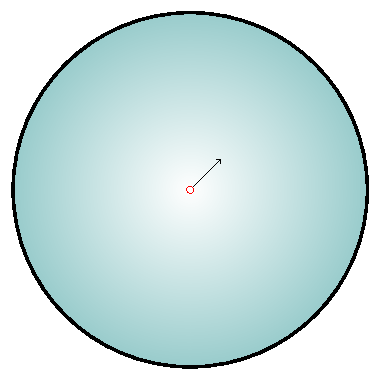
\includepdf[pages=-]{images/steps1.pdf}

\titre{Géodésiques, segments et droites}

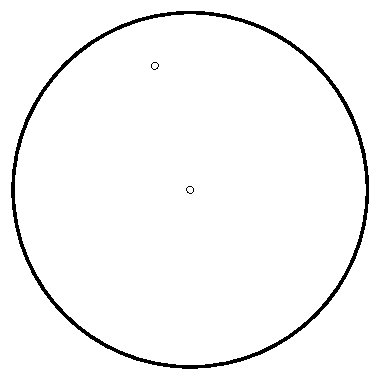
\includepdf[pages=-]{images/segments-droites.pdf}

\titre{Attention !!\\ Le 5ème postulat d'Euclide\\tombe en défaut!}

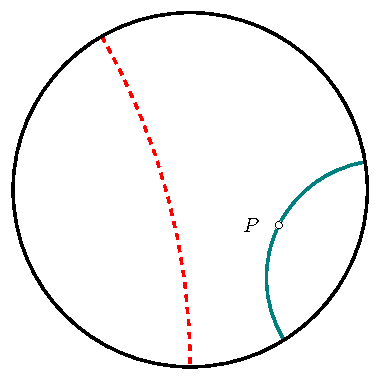
\includepdf[pages=-]{images/5eme-postulat.pdf}


\titre{Cercles}

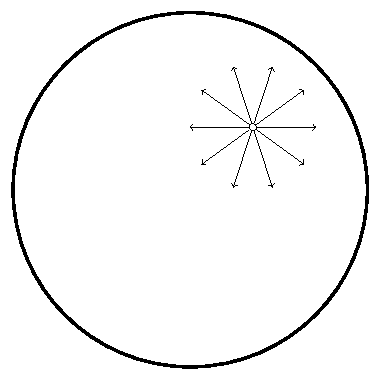
\includepdf[pages=-]{images/cercle.pdf}

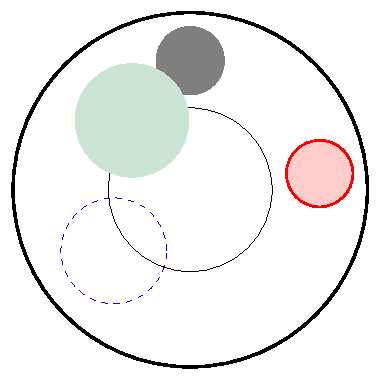
\includepdf[pages=-]{images/cercles-rayon-1.pdf}




\titre{Triangles:\\ Du normal et du moins normal}

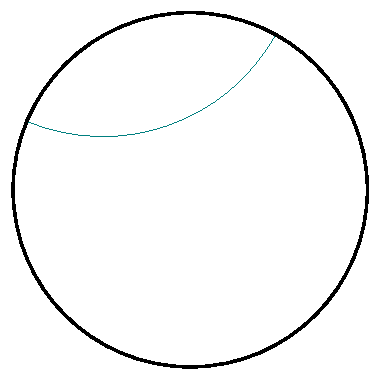
\includepdf[pages=-]{images/triangles.pdf}

\titre{Triangles:\\ Autres bizarreries\\ (Cercles circonscrits)}

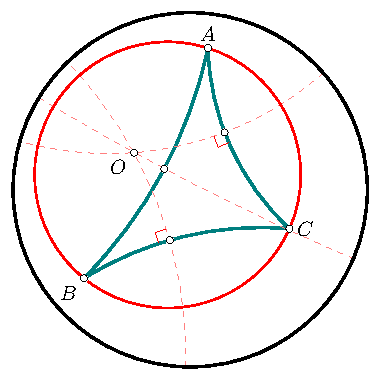
\includepdf[pages=-]{images/triangles-cercles-circonscrits.pdf}



\titre{Transformations (isométries)\\du plan hyperbolique}

\titre{Automorphismes elliptiques\\(Analogue des rotations)}


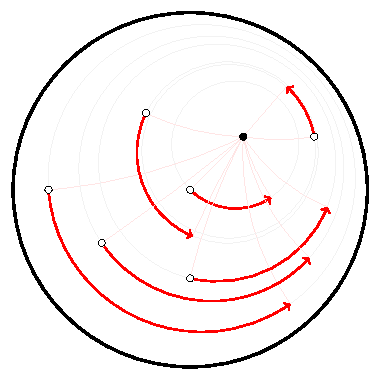
\includepdf[pages=-]{images/automorphismes-elliptiques.pdf}

\titre{Automorphismes hyperboliques\\(Analogue des translations)}

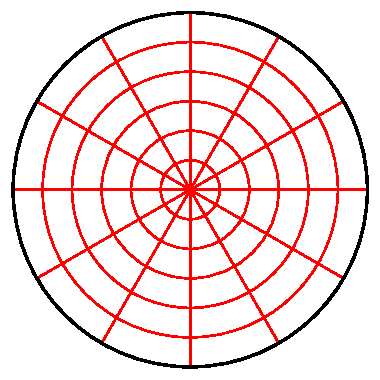
\includepdf[pages=-]{images/automorphismes-hyperboliques-anim.pdf}
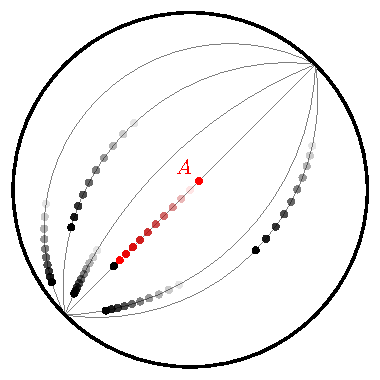
\includepdf[pages=-]{images/automorphismes-hyperboliques-orbites.pdf}

\titre{Automorphismes paraboliques\\(NON)}

\titre{Symétries axiales}

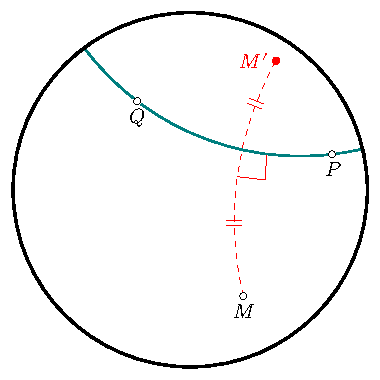
\includepdf[pages=-]{images/symetries-axiales.pdf}

\titre{Partie II\\ Programmer en  Lua\\dans un document (Lua)LaTeX}


\titre{Compilation avec lualatex\\  (plutôt que pdflatex)}

Très simple : \verb+lualatex myfile.tex+, ou \verb+latexmk --lualatex myfile.tex+.

Preambule minimal:

\begin{verbatim}
\documentclass{article}
\usepackage[french]{babel}
\usepackage{mathtools} % à charger avant unicode-math
\usepackage{unicode-math}  % charge fontspec
\end{verbatim}

Avantage immédiat (?) de la compilation avec LuaLaTeX choix de n'importe quelle police:

\begin{verbatim}
\setmainfont{Comic Sans MS}
Quelle indignité...
\setmainfont{Papyrus}
Je vous demande de vous arrêter !
\end{verbatim}

Pour plus d'informations sur les polices disponibles, voir les documents récents de Daniel Flipo :
\begin{itemize}
\item \url{https://danielflipo.fr/doc/luatex/pdf2lua.pdf}
\item \url{https://danielflipo.fr/doc/luatex/fonts.pdf}
\end{itemize}



\titre{Lua, un langage minimaliste\\  (Mais efficace!)}

\newpage

\vspace{1cm}


\begin{itemize}
\item Très simple à apprendre
\item Syntaxe très proche de Python (avec des \texttt{end} pour fermer les blocs)
\item site web : \url{lua.org}
\item Manuel : \url{https://www.lua.org/manual/}
\item Livre : \emph{Programming in Lua} (5ème édition, 1ère édition gratuite sur \url{https://www.lua.org/pil/contents.html}
\item Notes de cours : \url{https://ic.ufrj.br/~fabiom/lua/}
\item Utilisé dans un nombre croissant de packages latex, par exemple l'excellent \texttt{tkz-euclide}, pour augmenter la rapidité et la précision des calculs.
\end{itemize}

\newpage

\titre{Utilisation de Lua\\dans un document LaTeX}
%\setmathfont{Fira Math}
\begin{codeandresult}
La factorielle de $5$ vaut
\directlua{
	local result = 1
	for k=1,5 do result = result * k end
	tex.sprint(result)}.\par
La double factorielle de $5$,
notée $5!!$, est égale à 
\directlua{local n, result = 5, 1
	while n>0 do
		result = result * n
		n = n-2
	end
	tex.sprint(result)}.\par
La puissance de $2$ immédiatement
(strict°) supérieure à $100$ est 
\directlua{local n=1
	while n <= 100 do n = n * 2 end
	tex.sprint(n)}.
\end{codeandresult}

\newpage

%%%%%%%%%%%%%%%%%%%%%

%%%%%%%%%%%%%%%%%%%%%

%%%%%%%%%%%%%%%%%%%%%

\titre{Partie III\\ Quelques fonctionnalités\\du package `luahyperbolic'}

%%%%%%%%%%%%%%%%%%%%%

%%%%%%%%%%%%%%%%%%%%%

%%%%%%%%%%%%%%%%%%%%%

\paragraph{Informations pratiques} et liens

\begin{itemize}
\item Page CTAN : \url{https://ctan.org/pkg/luahyperbolic}
\item Repo github : \url{https://github.com/dmegy/luahyperbolic}
\end{itemize}

Attention, la version sur github est la plus à jour si l'on désire tester de nouvelles fonctionnalités.

\begin{center}
\begin{luacode*}
local PI = math.pi
local A, B, C = hyper.triangleWithAngles(PI/2, PI/4, PI/5)
local geodesics = {
	{hyper.endpoints(A,B)},
	{hyper.endpoints(B,C)},
	{hyper.endpoints(C,A)}
}
geodesics = hyper.propagateGeodesics(geodesics, 12) -- depth = 12
hyper.tikzBegin()
hyper.drawLinesFromTable(geodesics, "green!50!black, draw opacity=.5")
hyper.drawTriangle(A,B,C,"red, very thick")
hyper.tikzEnd()
\end{luacode*}
\end{center}

\newpage

\begin{codeandresult}
\begin{luacode*}
local A = -complex.I/2
local B = (1+complex.I)/2
local C = complex(-0.7,0.4)
local D = complex(-0.7,-0.3)
hyper.tikzBegin()
hyper.drawLine(A, B, "red")
hyper.drawSegment(B,C,"dashed, ForestGreen")
hyper.drawRay(C,D,"double,double distance=1pt")
hyper.drawLine(A,1,"gray,line width=2pt")
hyper.drawLine(1, complex.I, "teal")
hyper.drawPoints(A, B, C, D)
hyper.labelPoints(A, "$A$", B, "$B$", C, "$C$", D, "$D$")
hyper.tikzEnd()
\end{luacode*}
\end{codeandresult}

\newpage

\begin{codeandresult}
\begin{luacode*}
local A = complex(.9,.2)
local B = complex(.5,.7)
local C = complex(0,.9)
hyper.tikzBegin()
hyper.drawTriangle(A, B, C)
hyper.drawTriangle(-A, -B, -C, "red")
hyper.drawPolygon(-.9, -.7, complex(-.7,.4), complex(-.9,.3), "blue")
local points={}
for k=1,5 do
	table.insert(points, complex.polar(.4,k*2*math.pi/5))
end
hyper.drawPolygonFromTable(points,"teal")
hyper.tikzEnd()
\end{luacode*}
\end{codeandresult}

\newpage

\begin{codeandresult}
\begin{luacode*}
local A = -complex.I/2
local B = (1+complex.I)/2
local C = complex(-0.7,0.4)
local D = complex(-0.7,-0.3)
hyper.tikzBegin()
hyper.drawPolygon(A, B, C, D, "teal")
hyper.markSegment(A,B,"|")
local marking = "\\textcolor{red}{||}"
hyper.markSegment(B,C,marking)
hyper.labelSegment(C,D,"$3$", "fill=white, draw=blue")
hyper.labelSegment(D, A,"$\\alpha$", "below")
hyper.labelPoint(A, "$A$", "below")
hyper.tikzEnd()
\end{luacode*}
\end{codeandresult}

\newpage

\begin{codeandresult}
\begin{luacode*}
local theta=math.pi/3
local idealPoint = complex.exp_i(theta)
local N = 10
hyper.tikzBegin()
for k=1,N-1 do
	local point = idealPoint * (2*k/N-1)
	hyper.drawHorocycle(idealPoint,point,"red")
	-- and an orthogonal geodesic : 
	local endPoint = complex.exp_i(theta+2*k*math.pi/N)
	hyper.drawLine(idealPoint,endPoint,"gray")
end
hyper.tikzEnd()
\end{luacode*}
\end{codeandresult}

\begin{codeandresult}
\begin{luacode*}
hyper.tikzBegin()
local A = 1
local B = complex.J
hyper.drawLine(A,B,"very thick, teal")
local N = 10
for k=1,N-1 do
	local P = (2*k/N-1)*(-B^2)
	hyper.drawHypercycleThrough(P, A, B, "red")
end
hyper.tikzEnd()
\end{luacode*}
\end{codeandresult}

\newpage

\begin{codeandresult}
\begin{luacode*}
local A = complex(.4,.5)
local B = complex(-.5,0)
local AA, BB = hyper.endpoints(A,B)
hyper.tikzBegin()
hyper.drawSegment(A,B, "very thick, teal")
hyper.drawSegments(AA,A, B, BB, "dashed, red")
hyper.labelPoints(A, "$A$", B, "$B$")
hyper.labelPoint(AA, "$A'$", "red, below")
hyper.labelPoint(BB, "$B'$", "red, below right")
hyper.drawPoints(A, B)
hyper.drawPoints(AA,BB,"white, draw=red")
hyper.tikzEnd()
\end{luacode*}
\end{codeandresult}

\newpage

\begin{codeandresult}
\begin{luacode*}
local A = complex(0.4,0.6)
local B = complex(-0.8,-0.3)
local M = hyper.midpoint(A,B)
hyper.tikzBegin()
hyper.drawSegment(A,B, "very thick, teal")
hyper.drawPoints(A, B, M)
hyper.labelPoints(A, "$A$", B, "$B$")
hyper.labelPoint(M, "$M$", "below right, red")
local marking = "\\textcolor{red}{||}"
hyper.markSegment(A,M,marking)
hyper.markSegment(M,B,marking)
hyper.tikzEnd()
\end{luacode*}
\end{codeandresult}


\newpage

\begin{codeandresult}
\begin{luacode*}
local A = complex(0.4,0.3)
local B = complex(-0.4,-0.7)
local C = complex(0,0.7)
local D = complex(0.8,-0.4)
local P = hyper.interLL(A, B, C, D)
hyper.tikzBegin()
hyper.drawLines(A, B, C, D, "thick, teal")
hyper.drawPoints(A, B, C, D,"thick, teal")
hyper.drawPoint(P,"white, draw=red")
hyper.labelPoint(A, "$A$", "above")
hyper.labelPoint(B, "$B$")
hyper.labelPoint(C, "$C$", "left")
hyper.labelPoint(D, "$D$", "above")
hyper.labelPoint(P, "$P$", "left=.1cm, red")
hyper.tikzEnd()
\end{luacode*}
\end{codeandresult}
%
%\newpage
%
%\begin{codeandresult}
%\begin{luacode*}
%local A = complex(0.5,0.4)
%local B = complex(-0.3,-0.7)
%local O = complex(-0.4,0.2)
%local radius = 1.5
%local P, Q = hyper.interLC(A, B, O, radius)
%hyper.tikzBegin()
%hyper.drawLine(A, B, "teal")
%hyper.drawCircle(O,radius, "teal")
%hyper.drawSegments(O, P, O, Q, "red, dashed")
%hyper.drawPoints(A, B, O, "teal")
%hyper.drawPoints(P, Q, "white, draw=red")
%hyper.labelPoints(A, "$A$", B, "$B$", O, "$O$")
%hyper.labelPoints(P, "$P$", Q, "$Q$", "red, below right")
%local mark = "\\textcolor{red}{||}"
%hyper.markSegments(O, P, O, Q, mark)
%hyper.tikzEnd()
%\end{luacode*}
%\end{codeandresult}
%
%\newpage
%
%\begin{codeandresult}
%\begin{luacode*}
%local A = complex(-0.5,-.3)
%local B = complex(0.3,0)
%local r = hyper.distance(A, B)
%local P, Q = hyper.interCC(A, r, B, r)
%hyper.tikzBegin()
%hyper.drawCircle(A, r, "teal")
%hyper.drawCircle(B, r, "teal")
%hyper.drawPolygon(A, B, P, "dashed, red")
%hyper.drawPoints(P, Q, "white, draw=red")
%hyper.drawPoints(A, B, "teal")
%hyper.labelPoints(A, "$A$", B, "$B$", "below, teal")
%hyper.labelPoints(P, "$P$", "above left, red")
%hyper.labelPoint(Q, "$Q$", "red, below")
%local mark = "\\textcolor{red}{||}"
%hyper.markSegments(A, B, B, P, P, A, mark)
%hyper.tikzEnd()
%\end{luacode*}
%\end{codeandresult}

\titre{Pavages hyperboliques}
\begin{codeandresult}
\begin{luacode*}
local PI = math.pi
local DEPTH = 10
local A, B, C = hyper.triangleWithAngles(PI/3, PI/4, PI/5)
hyper.tikzBegin()
hyper.fillTilingFromTriangle(A, B, C, DEPTH)
-- default color is black
hyper.drawPolygon(A, B, C, "thick,red")
hyper.tikzEnd()
\end{luacode*}
\end{codeandresult}

\newpage



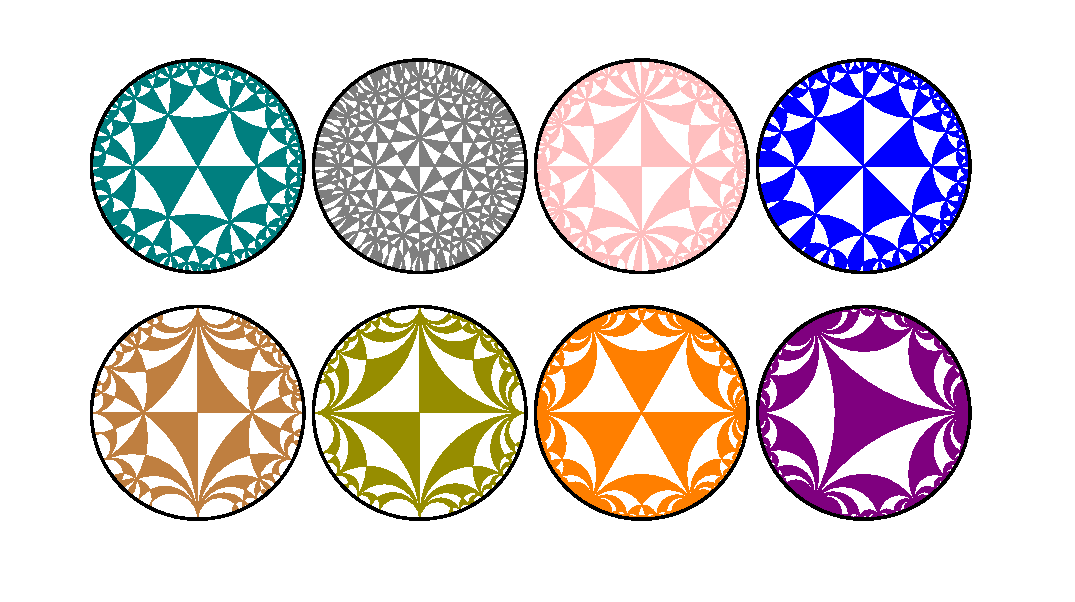
\includepdf[pages=-]{images/pavages.pdf}
%$ $\\
%
%\hyperbolicTiling{3}{4}{5}[scale=1.8, depth=6, color=teal]
%\hyperbolicTiling{2}{3}{7}[scale=1.8, depth=13, color=gray]
%\hyperbolicTiling{2}{5}{9}[scale=1.8, depth=7, color=pink]
%\hyperbolicTiling{4}{4}{4}[scale=1.8, depth=5, color=blue]
%
%\vspace{.5cm}
%\hyperbolicTiling{2}{5}{inf}[scale=1.8, depth=6, color=brown]
%\hyperbolicTiling{2}{inf}{inf}[scale=1.8, depth=6, color=olive]
%\hyperbolicTiling{3}{inf}{inf}[scale=1.8, depth=6, color=orange]
%\hyperbolicTiling{inf}{inf}{inf}[scale=1.8, depth=5, color=violet]

\begin{luacode*}
-- Print all entries of a given type in a module
function print_module_type(module, wanted_type, sep)
    sep = sep or ", "
    local names = {}
    for k, v in pairs(module) do
        if type(v) == wanted_type then
            table.insert(names, k)
        end
    end
    table.sort(names)
    for i, name in ipairs(names) do
        tex.sprint(-2, name)
        tex.sprint(sep)
    end

end
\end{luacode*}

\titre{Aperçu des fonctions disponibles}

\paragraph{Module `complex'} (petite lib de nombres complexes)
\ttfamily
\begin{multicols}{5}
\noindent\directlua{print_module_type(complex, "function", "\\\\")}
\end{multicols}

\newpage

\paragraph{Module `hyper'} (lib principale)

Attention, les fonctions préfixées par « \_ » vont peut-être redevenir privées donc non disponibles pour l'utilisateur. Il est demandé de ne pas les utiliser.

\ttfamily
\begin{multicols}{2}
\noindent\directlua{print_module_type(hyper, "function", "\\\\")}
\end{multicols}


\titre{Merci !\\ \vspace{1cm} \small{Dernière version et code source des slides : \\ \url{https://github.com/dmegy/expose-luahyperbolic-gutenberg-2026}}}

\end{document}